% !TEX root = main.tex

\section{集成学习}
集成学习(ensemble learning)通过构建并结合多个学习器来完成学习任务,通常可以获得比单一学习器更为显著的泛化性能。

同质(homogeneous)集成中的个体学习器称为基学习器(base learner);而异质(heterogeneous)集成中的个体学习器则一般称为组件学习器(component learner)。
\begin{figure}[H]
\centering
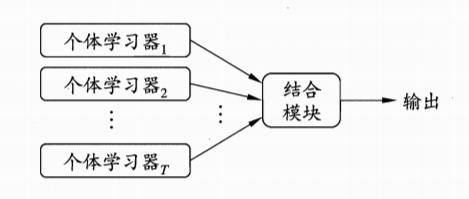
\includegraphics[width=0.5\linewidth]{fig/ensemble-learning.png}
\end{figure}

考虑二分类问题,假设基分类器的错误率为
\[\pr{h_i(\vx)\ne f(\vx)}=\eps\]
假设集成通过简单投票法结合$T$个分类器,若有超过半数的基分类器正确则分类正确
\[H(\vx)=\mathrm{sign}\lrp{\sum_{i=1}^Th_i(\vx)}\]
假设基分类器的错误率相互独立,则由Hoeffding不等式可得集成错误率为
\[\begin{aligned}
\pr{H(\vx)\ne f(\vx)}
&=\sum_{k=0}^{\lfloor T/2\rfloor}\binom{T}{k}(1-\eps)^k\eps^{T-k}\\
&=\exp\lrp{-\frac{1}{2}T(1-2\eps)^2}
\end{aligned}\]
即在一定条件下,随着集成分类器数目的增加,集成的错误率将指数级下降,最终趋于$0$。

但上面的分析有一假设:基学习器的误差相互独立。
现实生活中个体学习器是为解决同一个问题而训练出来的,显然不可能相互独立。
个体学习器的“准确性”和“多样性”之间本来就存在冲突。
如何产生“\textbf{好而不同}”的个体学习器是集成学习研究的核心。

\subsection{Boosting}
提升(Boosting)可以将弱学习器提升为强学习器,后面的模型是基于前面模型的训练结果(误差),个体学习器之间存在\textbf{强依赖关系},\textbf{串行生成},它的代表是AdaBoost。

\subsubsection{AdaBoost}
每一轮的训练集不变,只是训练集中每个样例在分类器中的\textbf{权重发生变化},而权值是根据上一轮的分类结果进行调整。
在每一步迭代中,会给训练集中的样本赋予权重$w_i$,样本的初始权重都一样为$1/n$。
每一步迭代中,被当前弱分类器\textbf{分错的样本权重会相应得到提高},被当前弱分类器分对的样本权重则降低(即刻意练习学得不好的样本),弱分类器的权重则由当前分类器的加权错误率来决定。

对目标函数$f(\vx)$进行多次逼近,通过不断拟合残差达到逼近的效果,可以按照下式不断迭代
\[\begin{aligned}
f_1(\vx) &=\widehat{f}(\vx)            & h_1(\vx) &=f(\vx)-f_1(\vx)\\
f_2(\vx) &=f_1(\vx)+\widehat{h_1}(\vx) & h_2(\vx) &=f(\vx)-f_2(\vx)\\
f_3(\vx) &=f_2(\vx)+\widehat{h_2}(\vx) & h_3(\vx) &=f(\vx)-f_3(\vx)\\
\vdots   &                             & \vdots \\
f_n(\vx) &=f_{n-1}(\vx)+\widehat{h_{n-1}}(\vx)
\end{aligned}\]

\begin{figure}[H]
\centering
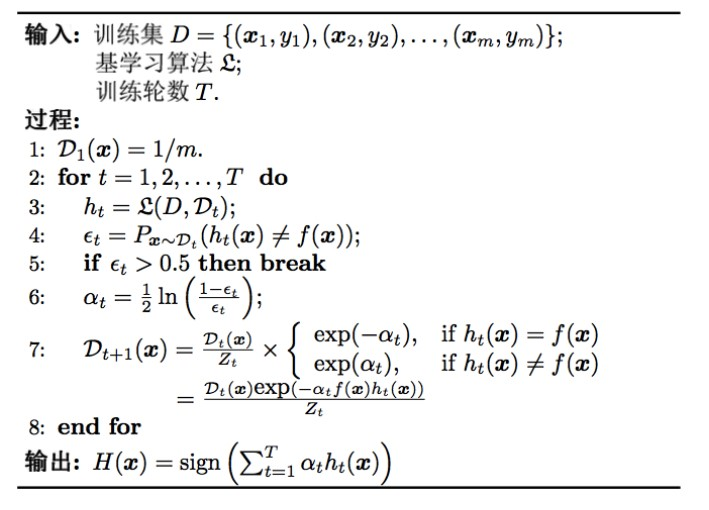
\includegraphics[width=0.8\linewidth]{fig/adaboost.jpg}
\caption{AdaBoost算法}
\end{figure}

\subsection{Bagging}
Bagging是Bootstrap aggregating的缩写,用来生成多个分类器并且集成这些分类器形成一个整体模型。
Bagging[Breiman, 1996]基于\textbf{自助采样法(有放回的随机采样)}\footnote{一个样本有$1-\frac{1}{n}$的概率不被选到,则一个样本不会被抽到的概率是$\lim_{n\to\infty}\lrp{1-\frac{1}{n}}^n=0.368$,意味着训练集包含63.2\%的不同样本。},采样出$T$个含$m$个样本的采样集$D_t$,然后基于每个采样集训练出一个基学习器$M_t$,再将这些基学习器结合。
对未知样本$X$分类,每个分类器返回类预测,直接\textbf{简单投票},将得票最高的类赋予$X$。
对于回归问题,则取每个分类器的预测值的\textbf{平均值}。

Bagging的时间复杂度低,与直接使用基学习器的复杂度同阶。
个体学习器\textbf{不存在强依赖关系}(意味着用什么不同类型的学习器都可以),可以\textbf{并行化生成}。

单个模型不稳定(轻微训练集的改变会造成分类器明显的变化,如决策树和神经网络),可以采用Bagging综合投票结果,提升稳定性及准确率。

\subsubsection{随机森林}
随机森林[Breiman, 2001]是Bagging的一个扩展变体。
传统决策树在选择划分属性时是在当前结点的属性集合(假定有$d$个属性)中选择一个最优属性;
而在随机森林中则是对基决策树的每个结点,先从该结点的属性集合中随机选择一个包含$k$个属性的子集,然后再从这个子集中选择一个最优属性进行划分。
这里的$k$即控制了随机程度,一般用$k=\log_2 d$[Breiman, 2001]。

为保证各棵树各不相同且预测结果\textbf{相互独立},随机森林中采用两到三层随机性:
\begin{enumerate}
	\item 随机有放回地抽取数据(使用Bagging)输入决策树模型
	\item 随机选取$k$个特征
	\item 随机选择特征取值进行分割(不遍历特征所有取值)
\end{enumerate}
注意由于建立决策树时的样本选择和特征选择所提供的随机性,因此不需要剪枝。

有两种指标衡量随机森林的表现:
\begin{itemize}
	\item 分类间隔(margin):森林中正确样本决策树的比例减去错误样本决策树的比例。
	假设样本$A$有75\%的树分类正确,那么分类间隔就是75\%-25\%=50\%。
	通常希望分类间隔越大越好,因为大的间隔表示我们的分类效果比较稳定,泛化效果更好。
	\item 袋外错误率(out-of-bag error):对每棵树来说,都有部分样本没有被抽样进入训练样本,这些即为袋外样本。
	随机森林对袋外样本的预测错误比率被称为袋外错误率。
	\begin{enumerate}
		\item 对每个样本,计算把该样本作为袋外样本的树对该样本的分类情况
		\item 以简单多数投票作为该样本的分类结果
		\item 用误分样本个数占样本总数的比率作为随机森林的袋外错误率
	\end{enumerate}
\end{itemize}

优点:
\begin{itemize}
\item 能够处理很高维数据,且不用做特征选择
\item 训练完可给出哪些特征比较重要
\item 容易做成并行化方法
\end{itemize}
缺点:相对于决策树,执行速度慢,模型可解释性较差

\subsection{Stacking}
最简单的就是简单平均或加权平均。
另外也可以通过投票法,绝对多数(majority)投票法、相对多数(plurality)投票法和加权投票法。

当训练数据很多时,更为强大的结合策略是使用学习法,即通过另一个学习器来进行结合。
Stacking [Wolpert, 1992]是学习法的典型代表。
这里把个体学习器称为次级学习器或元学习器(meta-learner)。

Stacking先从初始数据集中训练出初级学习器,然后\textbf{生成一个新数据集}用于训练次级学习器。
在新数据集中,初级学习器的输出被当作\emph{样例输入特征},而初始样本的标记仍被当作样例标记。
注意这个数据集的大小为$mT$,$m$为原数据集训练样本数,$T$为学习器数目。
\begin{figure}[H]
\centering
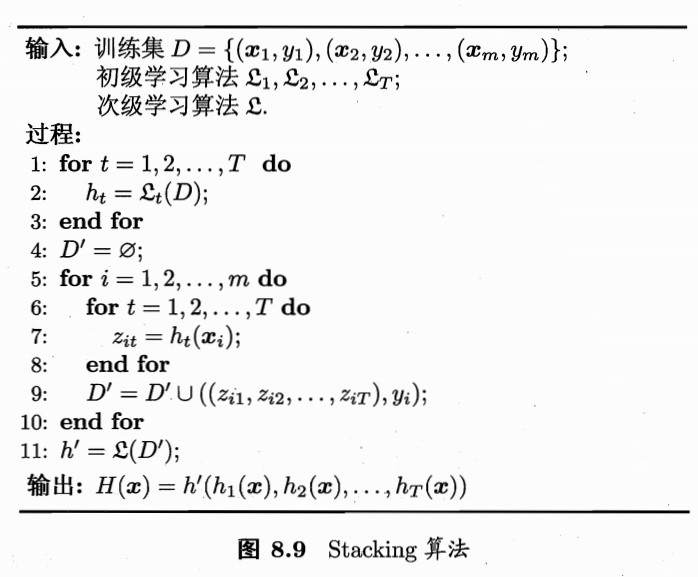
\includegraphics[width=0.6\linewidth]{fig/stacking.jpg}
\end{figure}

由于次级训练集是用初级学习器产生的,故直接用初级学习器的训练集产生次级学习器过拟合风险较大;因此常通过交叉验证或留一法,用训练初级学习器未使用的样本来产生次级学习器的训练样本。
以$k$折交叉验证为例,初始训练集$D$被随机划分为$k$个大小相似的集合$D_1,D_2,\ldots,D_k$。
令$D_j$和$\bar{D}_j=D\backslash D_j$分别表示第$j$折的测试集和训练集。
给定$T$个初级学习算法,初级学习器$h_t^{(j)}$通过在$\bar{D}_j$上使用第$t$个学习算法而得。
对于$D_j$的每个样本$\vx_i$,令$z_{it}=h_t^{(j)}(\vx_i)$,则由$\vx_i$所产生的次级训练样例的实例部分为$\vz_i=\bmat{z_{i1} & z_{i2} & \cdots & z_{iT}}$,标记部分为$y_i$。
故整个交叉验证过程结束后,从这$T$个初级学习器产生的次级训练集是$D'=\{(\vz_i,y_i\}_{i=1}^m$,然后$D'$将用于训练次级学习器。

总结Stacking的过程即:
\begin{enumerate}
\item 划分训练数据集为两(或多)个不相交的集合
\item 在第一个集合上训练多个学习器
\item 在第二个集合上测试这几个学习器
\item 把第三步得到的预测结果作为输入,把正确的回应作为输出,训练一个高层学习器
\end{enumerate}

% 贝叶斯模型平均(BMA)基于后验概率来为不同模型赋予权重,可视为加权平均的一种特殊实现。

\subsection{总结}
多样性增强的方法:
\begin{itemize}
	\item 数据样本扰动:通常基于采样法,Bagging中的自助采样法和AdaBoost中的序列采样。
	数据样本扰动对“不稳定基学习器”很有效。
	\begin{itemize}
		\item 对数据样本扰动敏感的不稳定基学习器:决策树、神经网络
		\item 对数据样本扰动不敏感的稳定基学习器:线性学习器、支持向量机、朴素贝叶斯、$k$近邻
	\end{itemize}
	\item 输入属性扰动:随机子空间算法,基于初始属性集,抽取出若干个属性子集,然后基于每个属性子集训练一个基学习器
\end{itemize}